\section*{Задача 3.2}
Дана разреженная матрица A. Найти число обусловленности матрицы.

\subsection*{Решение}
1. Зададим матрицу А согласно схеме из приложения: все ненулевые элементы матрицы равны $N$ ( номеру варианта), элементы главной диагонали равны  $N*m+m/N$,  $m$ - размерность матрицы.


\begin{verbatim}
A = np.eye(20, 20)
A[:8,:4] = N
A[8:14, 4:8] = N
A[14:, :8] = N
for i in range(8, m-1):
    A[i, i+1:] = N
for i in range(m):
    A[i, i] = (N*m + m/N)
\end{verbatim}

2.Разработаем и реализуем алгоритм решения системы с данной матрицей $А$ прямым методом с учетом нулевых элементов.
\begin{verbatim}
def zerofy(B, n):
    """Зануляет элеметны строки n, находящиеся под главной диагональю."""
    for i in range(0, n):
        mu = B[n, i] / B[i, i]
        B[n, :] -= mu * B[i, :]
    return B

def simplify(A, b):
    """Приводит разреженную матрицу А к двухдиагональному виду"""
    B = np.concatenate((A, b), axis = 1)
    for i in range(1, 8):
        B[i-1, :] -= B[i, :]
    for i in range(9, 20):
        B[i-1, :] -= B[i, :]
    B = zerofy(B, 7)
    B = zerofy(B, 13)
    B = zerofy(B, 19)
    return B[:, :-1], B[:, -1]

def backward(A, b):
    """Обратный ход для двухдиагональной матрицы"""
    x = np.zeros_like(b)
    x[-1] = b[-1] / A[-1, -1]
    for i in range(b.size-2, -1, -1):
        x[i] = (b[i] - A[i, i+1] * x[i+1]) / A[i, i]
    return x

def fast_solve(A, b):
    return backward(*simplify(A, b))
\end{verbatim}

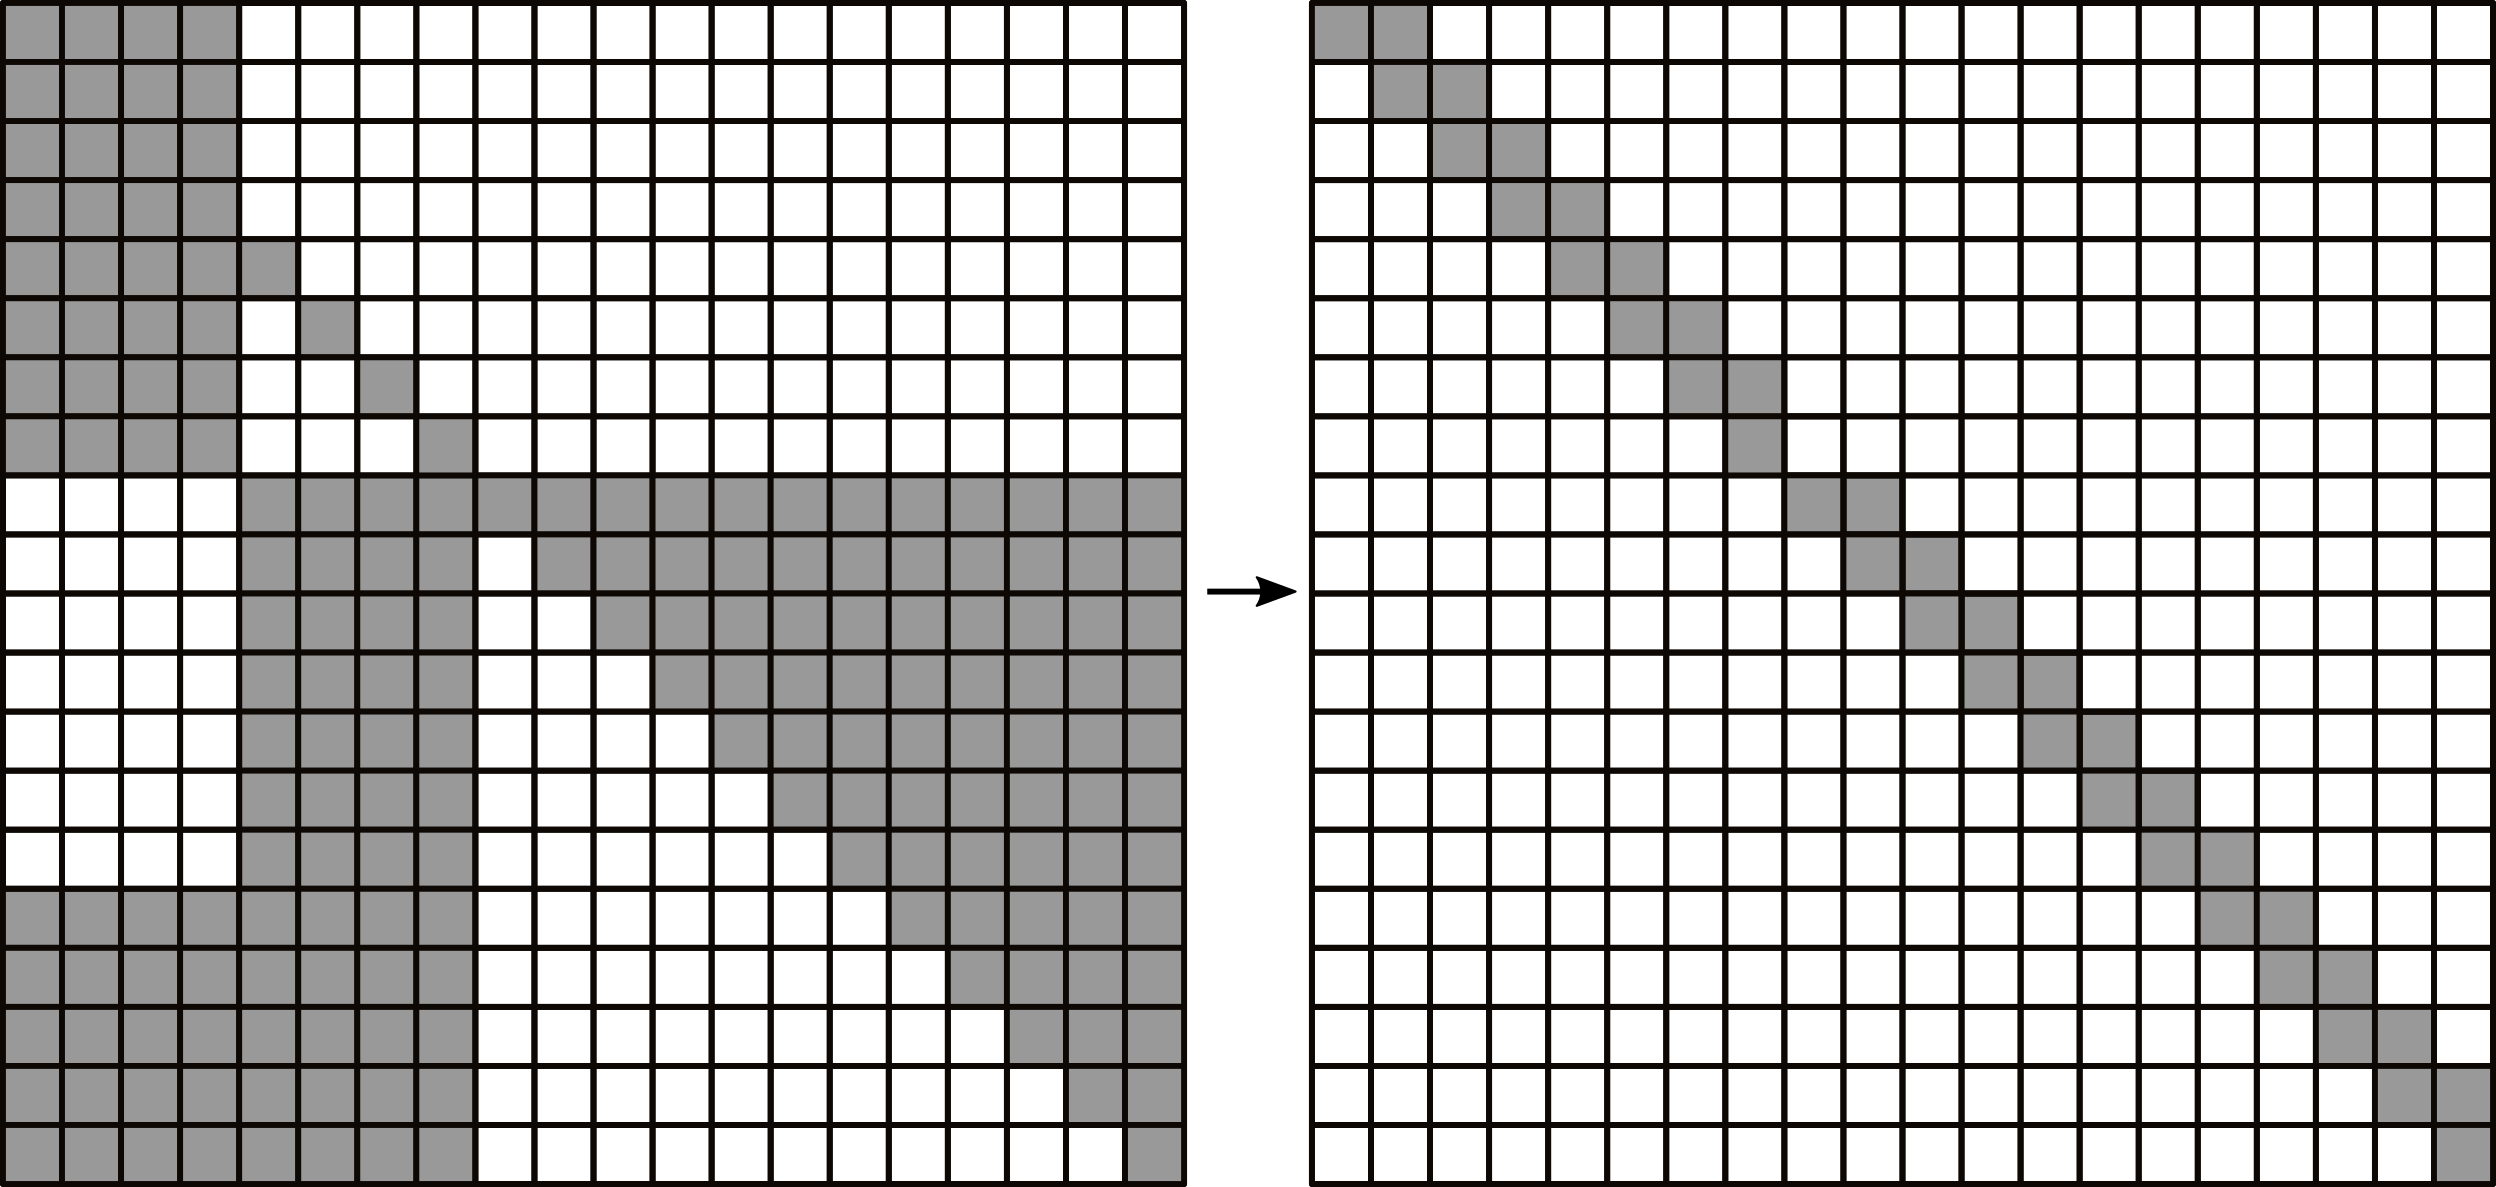
\includegraphics[width=15cm]{matr.png}

Выполним проверку, взяв вектор $x$, состоящий из одинаковых элементов $33$:
\begin{verbatim}
x_root = np.ones((20, 1)) * 33
b = A.dot(x_root)
fast_solve(A, b)

array([33., 33., 33., 33., 33., 33., 33., 33., 33., 33., 33.,
        33., 33., 33., 33., 33., 33., 33., 33., 33.])
\end{verbatim}

3. Напишим алгоритм для поиска обратной матрицы, основанный на решении уравнений $Ax^j=E^j$, где $E^j$ - столбцы единичной матрицы, проверим работоспособность:
\begin{verbatim}
def inv(A):
    ans = np.eye(*A.shape)
    for j in range(A.shape[1]):
        ans[:, j] = fast_solve(A, ans[:, j].reshape(A.shape[0], 1))
    return ans
\end{verbatim}

Проверим работоспособность алгоритма:

\begin{verbatim}
np.max(np.abs(inv(A).dot(A) - np.eye(20, 20)))

2.220446049250313e-16
\end{verbatim}


4. Найдем число обусловленности матрицы, используя евклидову норму:
\begin{verbatim}
condA = np.linalg.norm(A) * np.linalg.norm(inv(A))
condA

20.37275136439184
\end{verbatim}

5. Вывод

1. Данная матрица является хорошо обусловленной т.к. $cond A < 100$;

2. Трудоемкость метода составила:
   - 57m вычитаний, 3m умножений - функция simplify;

   - 3m вычитаний и умножений - функция backward;

   - Итого ~63m операций, т.е. сложность алгоритма - линейная.
